\documentclass{article}
\usepackage[margin=1in]{geometry}
\usepackage{graphicx}
\usepackage{amsmath}
\usepackage{multirow}
\usepackage{multicol}
\usepackage{wrapfig}



%\topmargin 0pt
%\oddsidemargin 12pt
%\evensidemargin 12pt
\interfootnotelinepenalty=10000


\begin{document}
\title{Partial Confidence in DNA Sequence Alignment}
\author{Yi Tian Xu\\260520039}

\maketitle

\abstract{}

%\begin{multicols}{2}

\section{Introduction}

% for simplicity, we consider linear gap

\subsection{Data}

A portion of CHR22, a predicted BoreoEutherian ancestor sequence, of 604,466 nucleotides was provided to us for the study and we use this data as the reference sequence. Each nucleotide $a$ in the sequence has an associated confidence value $p$ on the correctness of the prediction. We assume that each position in the sequence has equal chance of being one of the other three nucleotides if it were predicted wrong. 

\section{Method}

\subsection{Similarity measure}

Classical sequence alignment is based on a dynamic programming that computes some similarity measure for each pair of nucleotides of the input sequences. The similarity measure generally scores according to the likeness of the substitution, insertion and deletion. In our method, we use $m = 2$ for identity, $s_t = -1$ for transition and $s_v = -2$ for transversion substitutions, and a linear gap function $g(x)=-2x$. To formalize the substitution score, let $M$ be the substitution matrix. 
\begin{equation}
	M = \begin{bmatrix}
		m & s_v & s_t & s_v\\
		s_v & m & s_v & s_t\\
		s_t & s_v & m & s_v\\
		s_v & s_t & s_v & m\\
	\end{bmatrix}
\end{equation}
Given the alphabet $\Sigma =$ \{A,C,G,C\}, we can represent a nucleotide $a \in \Sigma$ as a vector $\vec{u}_a = (u_{\mbox{A}}, u_{\mbox{C}}, u_{\mbox{G}}, u_{\mbox{T}})$ where each entry $u_x = 1$ if $x = a$ or 0 otherwise. Thus, the score for matching two nucleotides, $a$ and $b$ can be formulate as $s(a,b) = \vec{u}_aM\vec{u}_b$.

To induce the probabilistic property in the reference sequence, we modify the similarity measure as the following. Given the reference nucleotide $a$ and its confidence probability $p$, we construct the vector $\vec{u}_{a,p} = (u_{\mbox{A}}, u_{\mbox{C}}, u_{\mbox{G}}, u_{\mbox{T}})$ where each entry $u_x = p$ if $x=a$ or $(1-p)/3$ otherwise. The score for matching a query nucleotide $b$ is $s(a,b,p) = \vec{u}_{a,p}M\vec{u}_b$. We can see that this preserves the scores in the total confidence setting since when $p=1$, $u_{a,p} = u_a$ for all $a \in \Sigma$. 

For the chosen parameters $m, s_t$ and $s_v$, Figure \ref{figure:score_graphs} shows the substitution score according to the variation in the confidence $p$. 

\begin{figure}[tbp]
\begin{center}
\caption{Substitution score variation according to the confidence value. When the confidence value is 1.00, the match, transition and transversion score reflect the case when the reference sequence is given with total confidence.}
   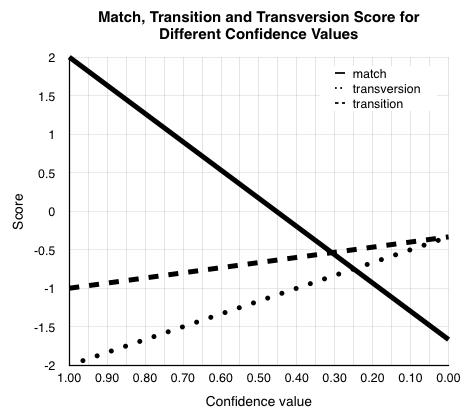
\includegraphics[width=0.50\textwidth]{score_graph}
\label{figure:score_graphs}
\end{center}
\end{figure}

\subsection{Database Indexing}

Smith-Waterman is unfeasible for aligning long sequence of millions of nucleotides. The standard heuristic to approach this problem is the basic local alignment search tool (BLAST) \cite{blast}. This method preprocesses the reference sequence $G$ by compiling a list of high-scoring $w$-mers. One can construct a hashtable keyed by all substrings of length $w$ in $G$ and valued by a list of the $w$-mers' occurred locations in $G$. Thus, the local alignment of a query sequence $q$ can be estimated at the locations in $G$ given by its $w$-mers that match the $w$-mers in $q$. When a matches, or hits, $h$ such that $q = q_1hq_2$ is found in the hashtable, BLAST subsequently perform the alignment of the prefix $q_1$ and suffix $q_2$ to obtain a complete alignment and score. The alignment with the highest score is then returned as best alignment.

In the context of partial confidence, we constructs the $w$-mers by treating all positions in the reference sequence with less than a certain confidence threshold, $\delta_p$, as a wildcard character. For example, for $w = 3$, a reference substring ``AAA" with confidences 1.00, 0.97 and 0.91 respectively expands to a set of 16 3-mers if $\delta_p > 0.97$ or 4 3-mers if $0.91 < \delta_p \leq 0.97$. 

This hashtable construction has two main issues. First, the running time for performing this construction has worst case $O(4^wL)$ where $L$ is the length of $G$. Depending on the distribution of the confidences, the method can be extremely inefficient for high $\delta_p$. In the case of our reference sequence, CHR22, Figure \ref{figure:conf_cum} shows the cumulative distribution of its confidence values. We observe a non-uniform distribution of the confidence values. In particular, around 80\% of the values are above 0.9, suggesting that a high confidence filtering threshold can be beneficial to the time efficiency of the method. 

The second issue is that low-scoring $w$-mers can be introduced to the database by a substring with uncertainty at multiple positions. It can be unclear to where the line of separation between low and high-scoring $w$-mers should be defined. Figure \ref{figure:score_dist} which show the observed distribution of scores for matching two sequences of lengths 3 and 7. We observe that both score distributions are unlikely to follow a normal distribution with 0 mean. Instead, a large portion of their weights tilt to the negative region, suggesting that a high-scoring $w$-mer may not necessarily score positively. Acknowledging the distribution, we attempt to investigate more on this issue experimentally by setting up a score threshold, $\delta_s$, which filters hits with scores less than $\delta_s$.

\begin{figure}[tbp]
\begin{center}
\caption{}
   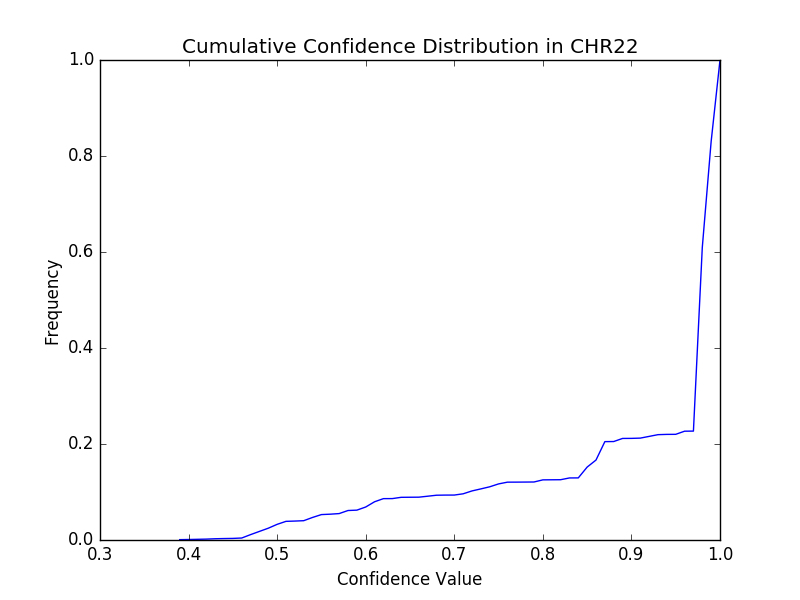
\includegraphics[width=0.49\textwidth]{conf-cum}
   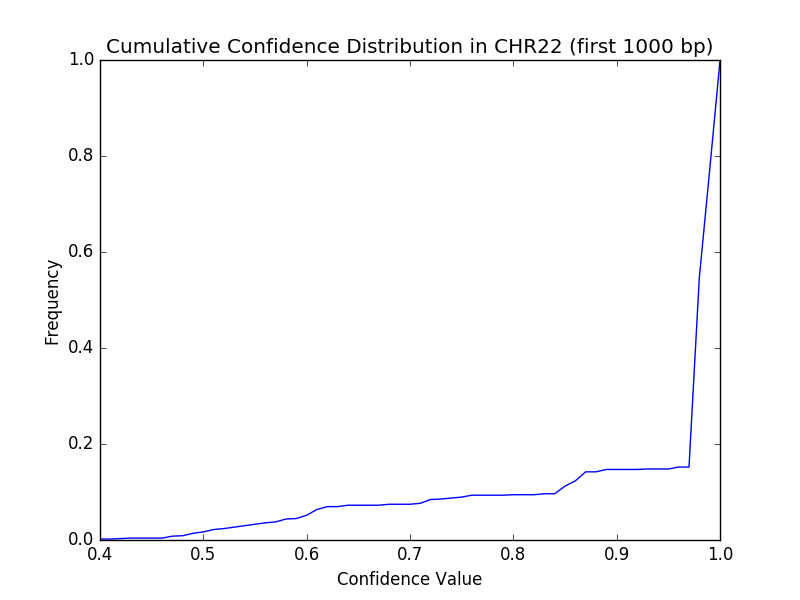
\includegraphics[width=0.49\textwidth]{conf-cum-1000}
\label{figure:conf_cum}
\end{center}
\end{figure}
\begin{figure}[tbp]
\begin{center}

\caption{Score distribution for $w \in \{3, 7\}$. The thicker line traces the observed score distribution for $w=7$, ranging between a score of $[-14, 14]$, which is sampled by randomly choosing 1000 words matching to a fixed words for each combination of confidence values formed with the set \{0.5, 0.75, 1\}. The lighter line corresponds to the case when $w=3$, ranging between of $[-6, 6]$, and we sampled similarity but using all the 64 words of length 3. Most scores lie on the negative side which suggests that a match with a positive score occurs rarely at random.}
   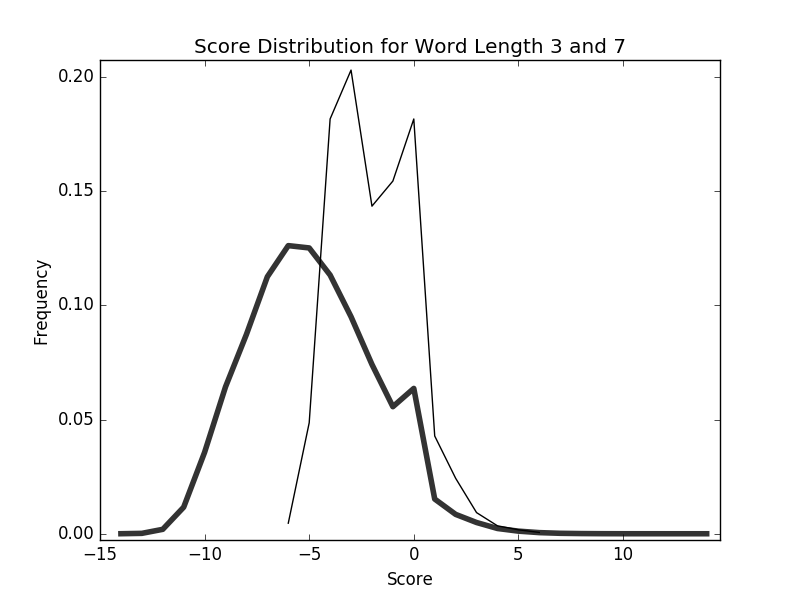
\includegraphics[width=0.60\textwidth]{score-dist}
\label{figure:score_dist}
\end{center}
\end{figure}

\subsection{Implementation}

Our implementation of partial confidence local search alignment has the following steps: (1) construct the database of $w$-mers for reference sequence, (2) for each $w$-mer in the query sequence, scan in the database for hits, (3) for each hit, run global alignment for the prefix and suffix of the query sequence, (4) return the alignment with the highest score. 

We use Hirschberg's algorithm for global alignment. This dynamic algorithm can has the advantage of performing in linear space, i.e.: $O(nm)$ where $n$ and $m$ are the lengths of the input sequences \cite{global_align}. We modified the open source Python software wuzhigang05/Dynamic-Programming-Linear-Space to match the similarity measures in our method. 

We allows certain simplification of the implementation, ignoring certain possibilities for optimization, without hindering the purpose of the experiment. One of such simplification applies to step (3). When aligning the prefix and suffix of a query sequence, we restrict the region of the reference sequence to which we want to align with in order avoid unnecessary insertion of gaps. The second simplification is on the size of the $w$-mers. As the optimal word size for constructing the database has been studied in other researches and may depend on the design of the indexing stage, we will not focus on this issue in our study. Instead, we conduct all our experiments with $w=7$ and focus on developing a mean for choosing of the confidence and score thresholds generalizable to all word size. 

\section{Experiment}

We test our implementation by aligning randomized substrings of length $w_q$ selected randomly from the CHR22 sequence. Our sequence randomization algorithm randomly induces at least $d$ substitutions and $g$ insertions and deletions to an input sequence. We compare the location $l_h$ to which a hit was found to the location $l_o$ where the substring was originally retrieved and considered the algorithm to have performed accurately if the output alignment outscores the alignment at the original location or if $|l_h - l_o| < w_q - w + g$. We consider output alignments that fail this condition ``suboptimal", and call query sequences with no hit found as ``no-hits".

This method allows us to obtain counts for the number of suboptimal alignments and of no-hits relative to the dissimilarity between the query sequence and the sequence where it originated from, which is defined by $w_q$, $d$ and $g$. 

\subsection{On the indexing confidence and score thresholds}

In this experiment, we study on the effect in the choice of the confidence and score thresholds, $\delta_p$ and $\delta_s$ respectively, for the indexing stage. In particular, we chose $\delta_p \in \{0.7, 0.8, 0.9\} $ and $\delta_s \in \{-13, -12, ... , 13\}$. Note that for a hit size of $w = 7$, with the substitution matrix $M$ of our choice, the lowest and highest hit scores are -14 and 14 respectively. As our implementation is not fully optimized, we use the first 1000 nucleotides of CHR22 as the reference sequence for the sake of time and space efficiency. As shown in Figure \ref{figure:conf_cum}, the cumulative distribution of the confidence values for this portion of the sequence is similar to the one for the entire sequence. Therefore, we assume that some of the results for this portion of the sequence can be generalized for the entire sequence.

For each $\delta_p$, we ran the experiment with $d \in \{2, 4\}$, $g \in \{0, 2, 4\}$ and $w_q \in \{10, 13, 15\}$. For each parameter settings, we sampled 1000 alignments using our sequence randomization algorithm. The same sample is used to test for each of the $\delta_s$.

\subsection{Local Alignment}

\section{Analysis}

From the result obtained from the experiment with the indexing confidence and score thresholds, we first analyze the impact of $\delta_s$ on the performance of the method. We observed that the occurrence of suboptimal alignment and no-hits is invariant when $\delta_s$ is small. As the threshold surpasses a certain value, the occurrence of suboptimal alignments starts decrease while the occurrence of no-hits beings to increase. For example, Figure \ref{figure:counts_10} shows the counts of suboptimal alignments and no-hits for $w_q = 10$ and $\delta_p = 0.9$, and we can see the transitions of the counts beginning around $\delta_s = 0$. We interpret this behaviour by the possibility that a significant portion of the low-scored $w$-mers lead to the suboptimal alignments, and are consequently excluded as $\delta_s$ grows larger, causing no more hits found for the previously suboptimally aligned query sequences. 

Another observation from Figure \ref{figure:counts_10} is that as the dissimilarity between the query sequence and the original sequence increases, the occurrence of suboptimal alignments and no-hits increases. An alternative way to reveal this trend is by comparing the percentage accuracy $A$ and hits $H$ which we defined as $A = 1 - \mbox{SUBOPTs}/(N - \mbox{NOHITs})$ and $H = 1 - \mbox{NOHITs}/N$ where SUBOPTs and NOHITs are the counts for suboptimal alignments and no-hits respectively, and $N$ is the number of samples. Figure \ref{figure:box_plot} plots the observed variability in the percentage accuracy and hits according to the different settings for $w_q$,  $d$ and $g$ in the randomization algorithm. In particular, the percentage accuracy appears to vary little compared to the percentage of hits. Notably, when dissimilarity of the query sequence increases ($d$ and $g$), the percentage of hits decreases dramatically, especially when increasing the number of insertions and deletions. Due to the nature of the randomization algorithm, certain location in the original sequence with confidence higher than $\delta_p$ might have been randomized, therefore they fail to lead to hits. We also observe in Figure \ref{figure:box_plots} that increasing the query sequence length $w_q$ can increase the percentage of hits. Perhaps, the most intuitive reason is that, due the small value of $w_q$ relative to $w$, an insertion or deletion can potentially destroy a location in the query sequence that would originally lead to a hit. 

Figure \ref{figure:big_page} plots the correlation between percentage accuracy and hits for each chosen $\delta_p$. We observe that there exists experiments with some particular set of $(w_p, d, g, \delta_s)$ in our samples that yields a high ($\ge$ 0.85) percentage of both accuracy and hits invariant of $\delta_p$. However, as drawn form the previous discussion, this behaviour is likely to occur with query sequence with low dissimilarity. Yet, this may suggest that as long as $\delta_p$ is reasonably high (say between 0.7 and 1.0), we can find an optimal alignment for a query sequence with $w_p > w$ that has enough resemblance to a portion of the reference sequence.

Figure \ref{figure:big_page} plots the correlation between percentage accuracy, hits and $\delta_s$ for each chosen $\delta_p$. As in Figure \ref{figure:counts_10}, the percentage accuracy and hits are invariant of $\delta_s$ when $\delta_s$ is small. Yet, the cutoff point that determines when variation begins may decrease as $\delta_p$ decreases. In this set of result, it may appear to lie between -3.5 and 3.5, which is half of $w$. 

To further investigate the choice of $\delta_s$, we plot the score frequency of the $w$-mers used to index the database for each $\delta_p$ (see Figure \ref{figure:hit_freq}) and observed that the score frequencies of $w$-mers with scores above 0 are relatively invariant to $\delta_p$ compared to the $w$-mers with scores below 0. This suggests that setting $\delta_s = 0$ may cause minor variation is the sets of $w$-mers used to index the database if we need to change $\delta_p$. It may also suggests from a practical perspective that the size of the database 

\begin{figure}[tbp]
\begin{center}
\caption{}
  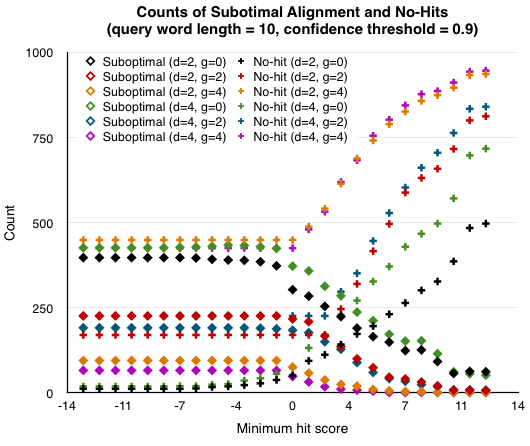
\includegraphics[width=0.60\textwidth]{counts-10}
  \label{figure:counts_10}
\end{center}
\end{figure}


\begin{figure}[tbp]
\begin{center}
\caption{}
   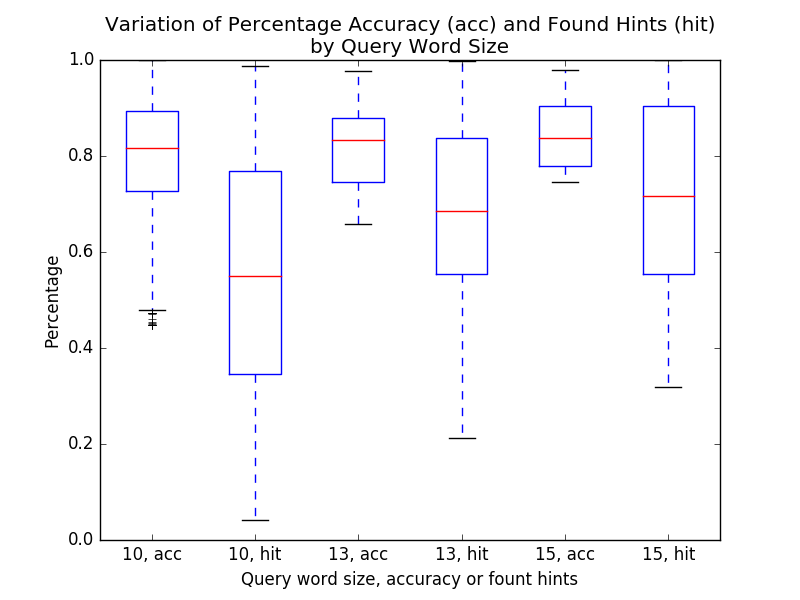
\includegraphics[width=0.49\textwidth]{size}
   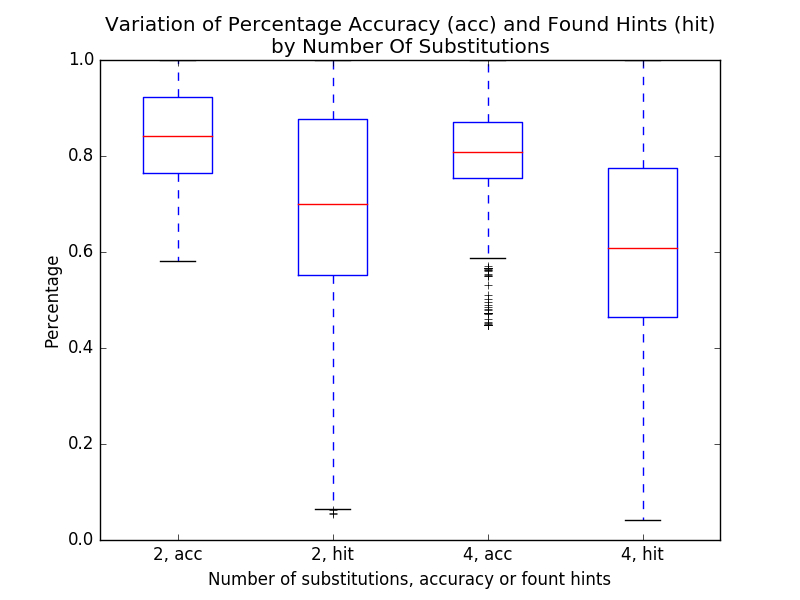
\includegraphics[width=0.49\textwidth]{diff}
   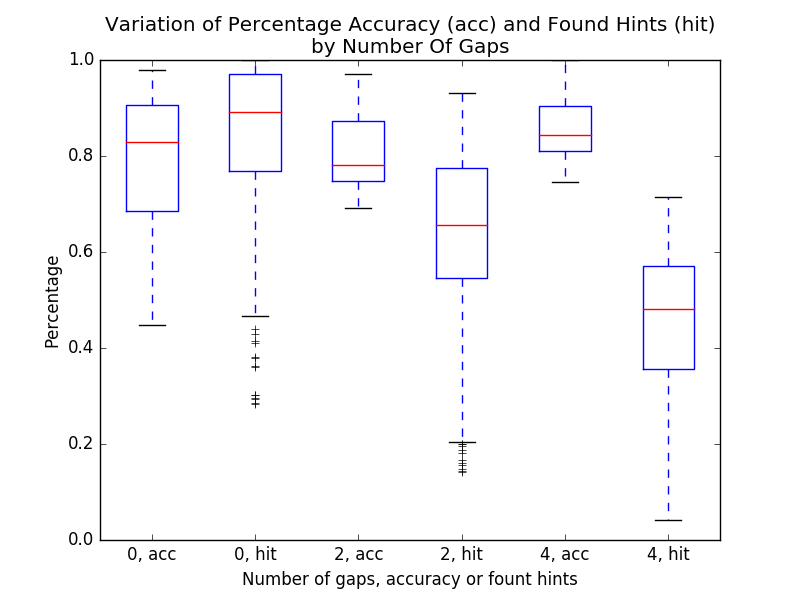
\includegraphics[width=0.49\textwidth]{gap}
   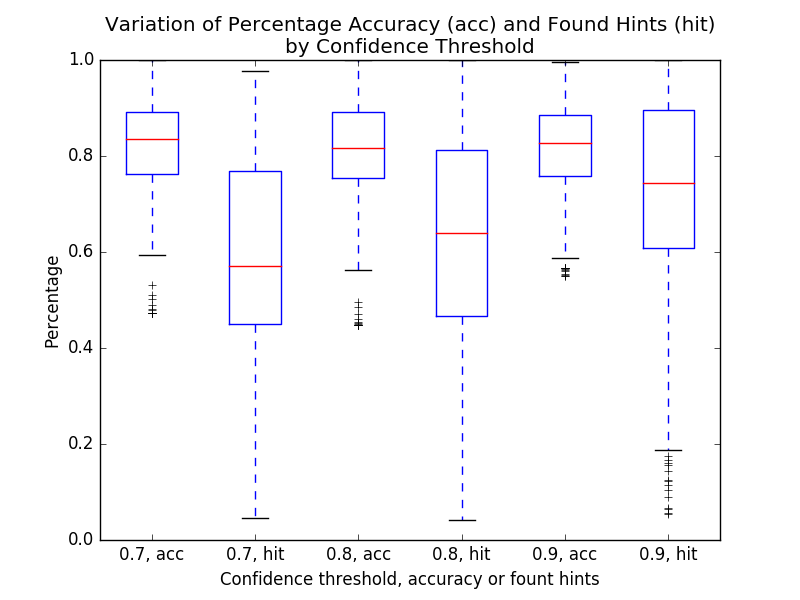
\includegraphics[width=0.49\textwidth]{conf}
\label{figure:box_plots}
\end{center}
\end{figure}


\begin{figure}[tbp]
\begin{center}
\caption{}
  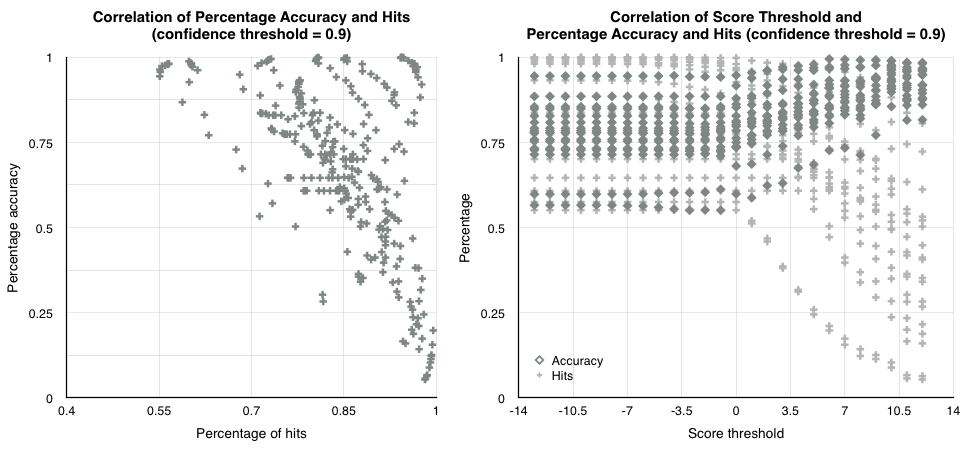
\includegraphics[width=0.99\textwidth]{09}
   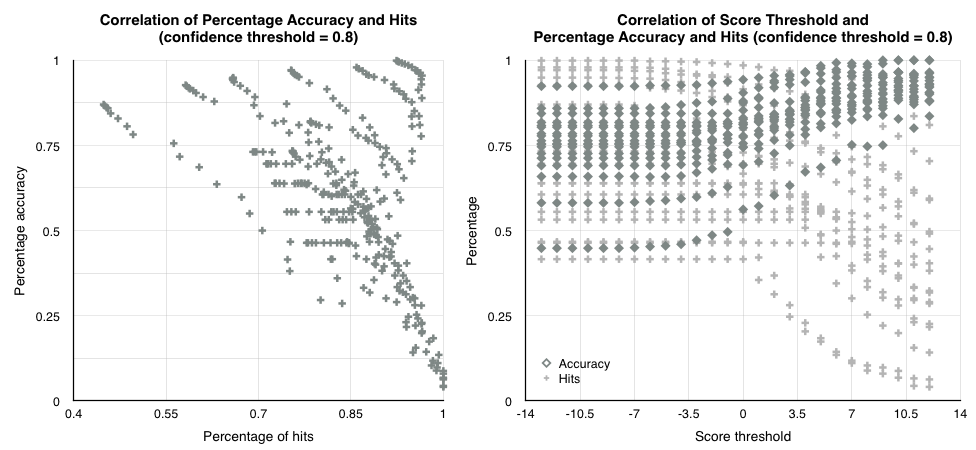
\includegraphics[width=0.99\textwidth]{08}
   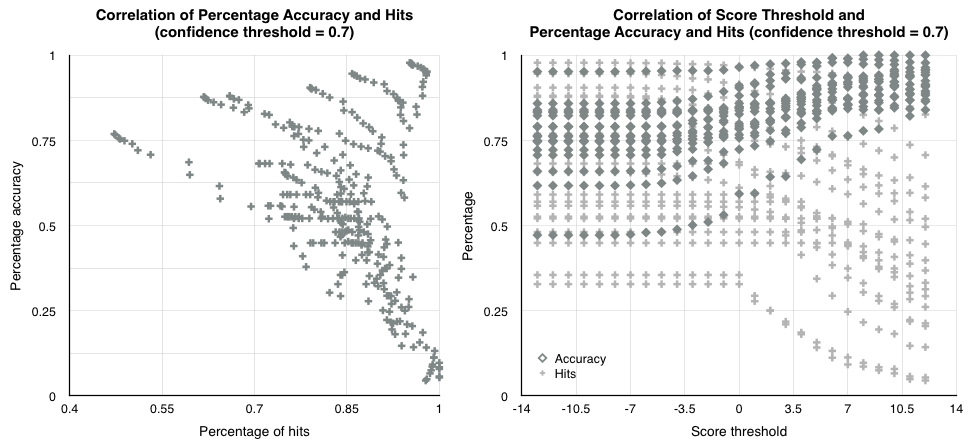
\includegraphics[width=0.99\textwidth]{07}
\label{figure:big_page}
\end{center}
\end{figure}

\begin{figure}[tbp]
\begin{center}
\caption{}
  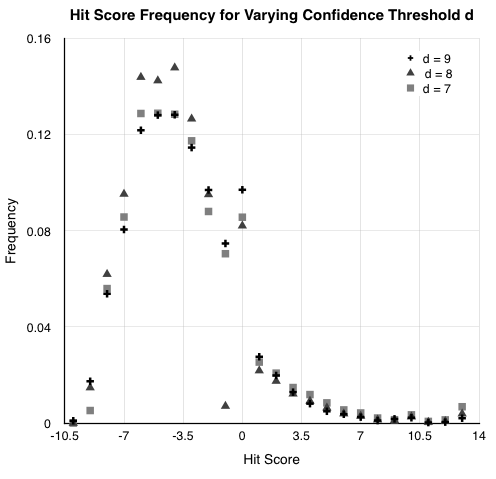
\includegraphics[width=0.60\textwidth]{hit-score-freq-1000}
\label{figure:hit_freq}
\end{center}
\end{figure}

\begin{thebibliography}{9}

\bibitem{blast}
	Stephen F. Altschu et al,
	Basic Local Alignment Search Tool.
	J. Mol. Biol. (1990) 215, 403-410 
	
\bibitem{global_align}
  Zhigang Wu,
  wuzhigang05/Dynamic-Programming-Linear-Space,
  (2013),
  Github Repository,
  https://github.com/wuzhigang05/Dynamic-Programming-Linear-Space

\end{thebibliography}
%\end{multicols}
\end{document}